
\section{提高效率和效果}

提高联邦学习的效率和效果
\begin{enumerate}
    \item 开发更好的优化算法;为不同的客户提供不同的模型;
    \item 使ML任务, 如超参数搜索、架构搜索和调试在FL上下文中更容易;
    \item 提高沟通效率
\end{enumerate}

\subsection{挑战一--联邦学习中的非独立同分布数据}
现有的机器学习任务默认训练数据遵循独立同分布, 神经网络常见算法一般都将数据遵循IID的假设作为其推导的一部分.但是, 在真实世界中样本数据相关性几乎无处不在, 非同源数据/标签的分布也可能具有不同的概率分布, 这些数据都遵循非独立同分布.
在一些场景中, 直接应用已有机器学习算法基于 Non-IID 数据完成模型训练, 由于算法本身的先进性训练结果仍然较好.但对于某些应用场景, 基于现有的机器学习算法和框架, 使用 Non-IID 数据训练会出现意想不到的负面效果, 比如模型准确度低、模型无法收敛等.
比较常见的需要处理 Non-IID 数据问题的应用场景包括:异常检测(Outlier Detection)、生物医学应用(Medical Data)、联邦学习 (Federated Learning).

在联邦学习的应用场景中, 各个设备上的数据是由设备/用户独立产生的, 不同设备/用户的非同源数据具有不同的分布特征, 而每一个设备在进行本地学习的时候, 所学习的训练数据是 Non-IID 的.因此研究提升 Non-IID 数据的学习效率, 对于联邦学习具有重要意义.联邦学习允许用户在不需要集中存储数据的情况下, 从本地存储的数据中共同获得共享模型的好处.客户端的本地数据通常基于特定用户对移动设备的使用, 因此任何特定用户的本地数据集都不能代表总体分布.


依赖和非同质性的最常见来源是对应于特定用户、特定地理位置和/或特定时间窗口的每个客户机.这种分类法与数据集移位的概念有密切的关系,  其中研究了训练分布和测试分布之间的差异;这里, 我们考虑每个客户机上数据分布的差异.

以下, 考虑一个监督任务特征x和y标签.联邦学习的的统计模型, 给出学习包括两个层次的抽样:访问一个数据需要首先采样一个客户$i\sim Q$, 客户可用的分布, 然后画一个例子$(x,  y) \sim P_i(x,  y)$从客户机的本地数据分布.

当引用联合学习中的非iid数据时, 这通常是指Pi和Pj对于不同的i和j客户机的差异.然而, 值得注意的是, 分布$Q$和$Pi$可能会随着时间的变化而变化, 从而引入另一个“non-iidness”维度.

为了完整性: 单个设备上的数据集,  独立性在局部也可能会被破坏, .例如, 视频中连续的帧是高度相关的.客户端内部相关性的来源通常可以通过\textbf{局部变换}来解决.

\paragraph{非同质的客户端分布}
数据偏离同分布的方式\citep{hsieh2019non},     $P_i \neq P_j$ 代表不同客户端 $i$ and $j$. 用 $P_i(y | x) P_i(x)$ and $P_i(x | y) P_i(y) $重写$P_i(x,  y)$, 这样可以更精确地描述不同.
\begin{description}
    \item[特征分布倾斜] 即使$P(y, j, x)$相同,  $P_i(x)$的边际分布在不同的客户端之间也可能不同
    \item[标签分布倾斜] 即使$P(x,  j,  y)$是相同的, $P_i(y)$的边际分布在不同的客户端可能是不同的.
    \item[标签相同, 特征不同] 即使 $P(y)$相同,  $Pi(x, j, y)$的条件分布在不同的客户机上也可能不同.
    \item[特征相同, 标签不同] 即使$P(x)$是相同,  条件分布$Pi(y, j, x)$在不同的客户端可能不同, .
    \item[数量倾斜或不平衡]不同客户端拥有不同数量数据.
\end{description}

此外, 不同的non-iid方式可能需要制定不同的应对策略.例如, 由于假定$P(y | x)$是常见的, 所以在特征分布倾斜的情况下, 至少在原则上详细说明了这个问题, 并且训练一个学习$P(y | x)$的全局模型可能是适当的.当相同的特性映射到不同客户端上的不同标签时, 可能需要训练某种形式的个性化模型.

\paragraph{违反独立性}
在训练过程中, 一旦分布Q发生变化, 就会出现违反独立性的情况.一个例子是跨设备FL中设备通常需要满足资格要求才能参加训练.设备通常在夜间本地时间满足这些要求(当它们更有可能在充电、使用免费wi-fi和空闲时), 因此设备可用性可能存在明显的昼夜变化模式.此外, 由于当地时间与经度直接相关, 这就在数据来源中引入了很强的地理偏差.Eichner等人[151]描述了这个问题和一些缓解策略, 但仍有许多悬而未决的问题.

\paragraph{数据集偏移}
Q和P分布的时间依赖性可能会引入经典意义上的数据集偏移(训练分布和测试分布之间的差异).此外, 其他条件可能会使有资格训练联合模型的客户端集合不同于将部署该模型的客户端集合.例如, 训练可能需要比推理所需内存更多的设备.


%将处理数据集的技术转换为联邦学习是另一个有趣的开放问题.
\subsubsection{解决non-IID Data 问题的策略}
联合学习的最初目标是在客户端数据集的联合上训练单个全局模型, 但对于non-iid数据, 这一目标更难实现.一种自然的方法是\textbf{修改现有的算法(例如通过不同的超参数选择)或开发新的超参数}以更有效地实现这一目标.
对于某些应用程序, 可能需要增加数据以使跨客户机的数据更加相似.一种方法是\textbf{创建一个可以全局共享的小数据集}.该数据集可能来自一个公开可用的代理数据源, 一个独立于客户端数据的不隐私敏感的数据集, 或者可能是原始数据的提炼.客户目标函数的异构性使得如何构建目标函数的问题变得更加重要——现在已经不清楚是否对所有示例都同等看待.
multi-model
替代选择包括\textbf{限制来自任何一个用户的数据贡献}, 并\textbf{在客户端之间引入公平}的概念.但是, 如果我们能够在每个设备上的本地数据上运行训练(这对于全局模型的联合学习是必要的), 那么训练单个全局模型是否是正确的目标呢?
在许多情况下, 最好使用单个模型, 例如为了向没有数据的客户端提供模型, 或者为了在部署之前允许手工验证和质量保证.然而, 由于本地训练是可能的, 因此每个客户都有一个定制的模型是可行的.这种方法可以把非iid问题从一个bug变成一个特性, 几乎是字面上的意思——因为每个客户端都有自己的模型, 客户端的身份有效地参数化了模型, 使一些病态但退化的非iid分布变得微不足道.例如, 如果对于每一个$i,  Pi(y)$仅在一个标签上有支持, 那么找到一个高精度的全局模型可能是非常具有挑战性的(特别是当x的信息相对不足时), 但是训练一个高精度的局部模型是不重要的(只需要一个恒定的预测).
除了解决不相同的客户端之外, 使用多个模型还可以解决由于客户端可用性变化而导致的独立性违背问题.
\subsection{联邦学习的优化算法}
在典型的联邦学习任务中, 目标是学习单个全局模型, 该模型最小化整个训练数据集上的风险函数, 即所有客户机的数据联合.联邦优化算法和分布式训练方法之间的主要区别是, 对于优化, non-iid和不平衡数据、有限的通信带宽、不可靠的和有限的设备可用性是特别突出的.

FL设置中, 设备的总数是巨大的(例如跨移动设备), 这就要求算法每轮只需要少量的客户端参与(客户端抽样).此外, 每个设备在给定模型的训练中可能只参与一次, 因此无状态算法是必要的.这就排除了直接应用在数据中心环境中非常有效的各种方法, 例如ADMM之类的有状态优化算法, 以及根据前几轮遗留的压缩错误修改更新的有状态压缩策略.
联邦学习算法的另一个重要的实际考虑是与其他技术的可组合性.优化算法不会在生产部署中单独运行, 但需要与其他技术相结合, 如加密的安全聚合协议、差异隐私(DP)和模型和更新压缩.这些技术可以应用于原语“选中求和客户”和“广播选择客户”, 所以表达这些原语方面的优化算法提供了一个宝贵的关注点分离, 但也可能排除某些技术, 如异步应用更新.
最常见的一种优化方法对于联邦学习是联邦平均算法\citep{mcmahan2016communication}, 采用local-update或parallel SGD.这里, 每个客户端运行在本地一些SGD步骤, 然后更新本地模型平均形成协调服务器上更新全局模型.伪代码在算法1中给出.执行本地更新并减少与中央服务器的通信频率, 解决了尊重数据位置约束和移动设备客户端有限通信能力的核心挑战.然而, 从优化理论的角度来看, 这类算法也带来了一些新的算法挑战. 开发专门针对联邦学习设置特征的新算法仍然是一个重要的开放问题.
\begin{figure*}[ht]
    \setlength{\abovecaptionskip}{0.1cm}
    \centering
    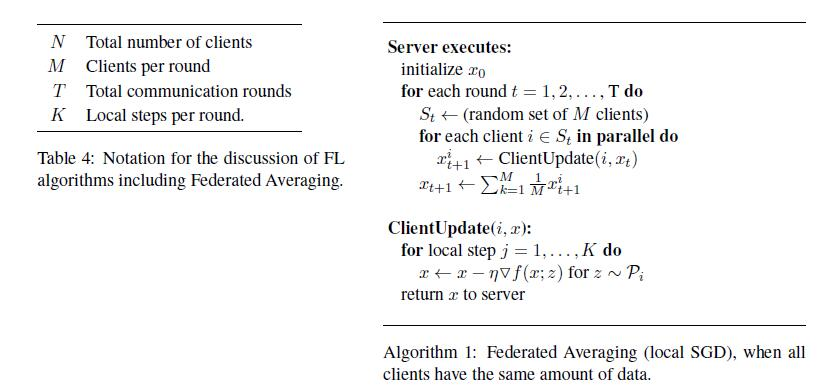
\includegraphics[width=0.9\textwidth]{Federated_Averging.jpg}
    \caption{联邦平均算法}
\end{figure*}

\subsubsection{ IID数据集的优化算法和收敛速度}

虽然可以对正在优化的每个客户端函数进行各种不同的假设, 但最基本的划分是假设IID和非IID数据.在形式上, 在客户端拥有IID数据意味着用于客户端本地更新的每一小批数据在统计上与从整个训练数据集中(客户端所有本地数据集的联合)一致绘制的样本(带有替换)相同.由于客户独立地收集他们自己的培训数据, 这些数据在大小和分布上都有所不同, 而且这些数据不与其他客户或中心节点共享, 因此IID的假设在实践中几乎不可能成立.然而, 这个假设极大地简化了联邦优化算法的理论收敛分析, 并建立了一个基线, 可以用来理解非IID数据对优化率的影响.因此, 自然的第一步是了解IID数据案例的优化算法.

% Communication-Efficient Learning of Deep Networks from Decentralized Data
% \citep{mcmahan2016communication}

% Federated Learning with Non-IID Data 
% \citep{zhao2018federated}